\section{Experimental Results}

\subsection{Implementation}

\begin{figure}[!ht]
\begin{center}
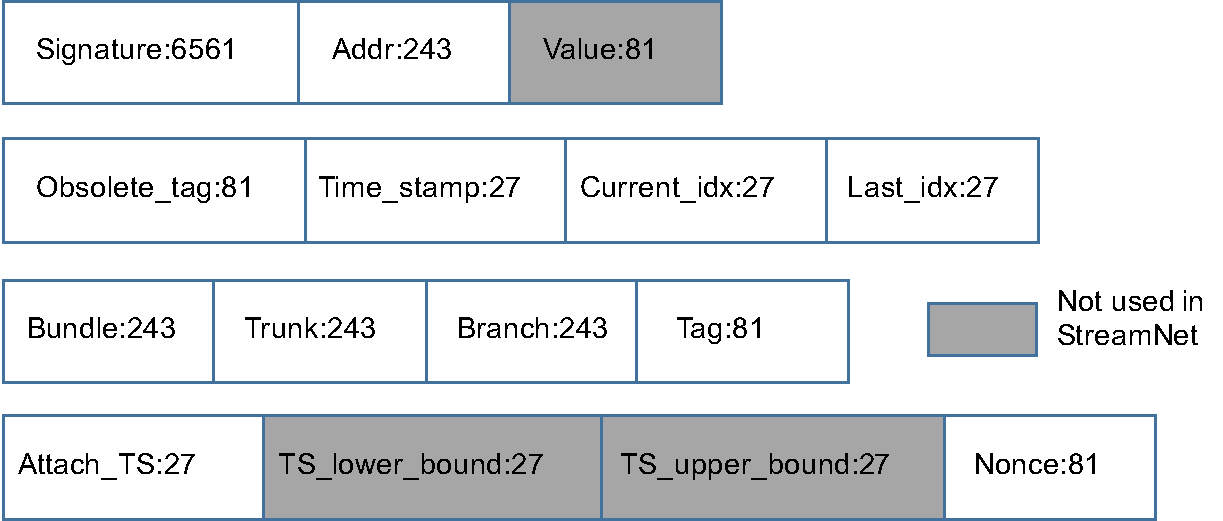
\includegraphics[width=0.45\textwidth]{figures/block_format.pdf}
    \caption{
        Block header format, the main transaction information is stored in the signature part. Addr is sender's address, time stamp is the time the block has been created, current/last index and the bundle are used for storing the bundle information, trunk and branch are the hash address to store the parent and reference location, tag is used for store some tagging information, addtach\_TS is when the block is attached to the StreamNet, nonce is used in POW calculation.
     }
\label{block_header}
\end{center}
\end{figure}

We have implemented the StreamNet based on the IOTA JAVA reference code (IRI) v1.5.5 \cite{IOTACode}.
We forked the code and made our own implementation, the code is freely available at \cite{StreamNet}.
In this paper we use version v0.1.4-streamnet in v0.1-streamnet beta branch.

\begin{itemize}
    \item The features we have adopted from the IRI are: 
    \begin{itemize}
        \item The block header format, as shown in Figure~\ref{block_header}. Some of the data segments are not used in StreamNet which are marked grey.
        \item Gossip network, the network is a bi-directional network in which every node will send and receive data from its peers;
        \item Transaction bundle, because of the existence of the bundle hash feature, StreamNet can support both the single transaction for a block and batched transactions as a bundle. 
        \item Sponge hash functions which is claimed to be quantum immune, in our experiment, the POW hardness is set to 8 which is the same as the testnet for IOTA.
    \end{itemize}

    \item The features we have abandoned from the IRI are:
    \begin{itemize}
        \item The iota's transaction logic including the ledger validation part;
        \item The milestone issued by coordinators, which is a centralized set up. 
    \end{itemize}

    \item The features we have modified based on the IRI is: 
    \begin{itemize}
        \item The tip selection method based on MCMC, since the tip selection on IRI has to find a milestone to start searching, we replace this with a block in the pivotal chain instead.
    \end{itemize}


    \item The features we have added into the StreamNet are: 
    \begin{itemize}
        \item The consensus algorithms, and we have applied the streaming method directly in the algorithms; 
        \item The UTXO logic which is stored in the signature part of the block header, we used the graph data structure to store UTXO as well. 
        \item In IOTA's implementation, the blocks are stored in the RocksDB \cite{RocksDB} as the persistence layer, which makes it inefficient to infer the relationships between blocks and calculate graph features. In our implementation, we introduced an in-memory layer to store the relationships between blocks, such that the tip selection and total ordering algorithm will be accelerated. 
    \end{itemize}
\end{itemize}

\subsection {Environment Set Up}

\begin{figure*}[!ht]
\begin{center}
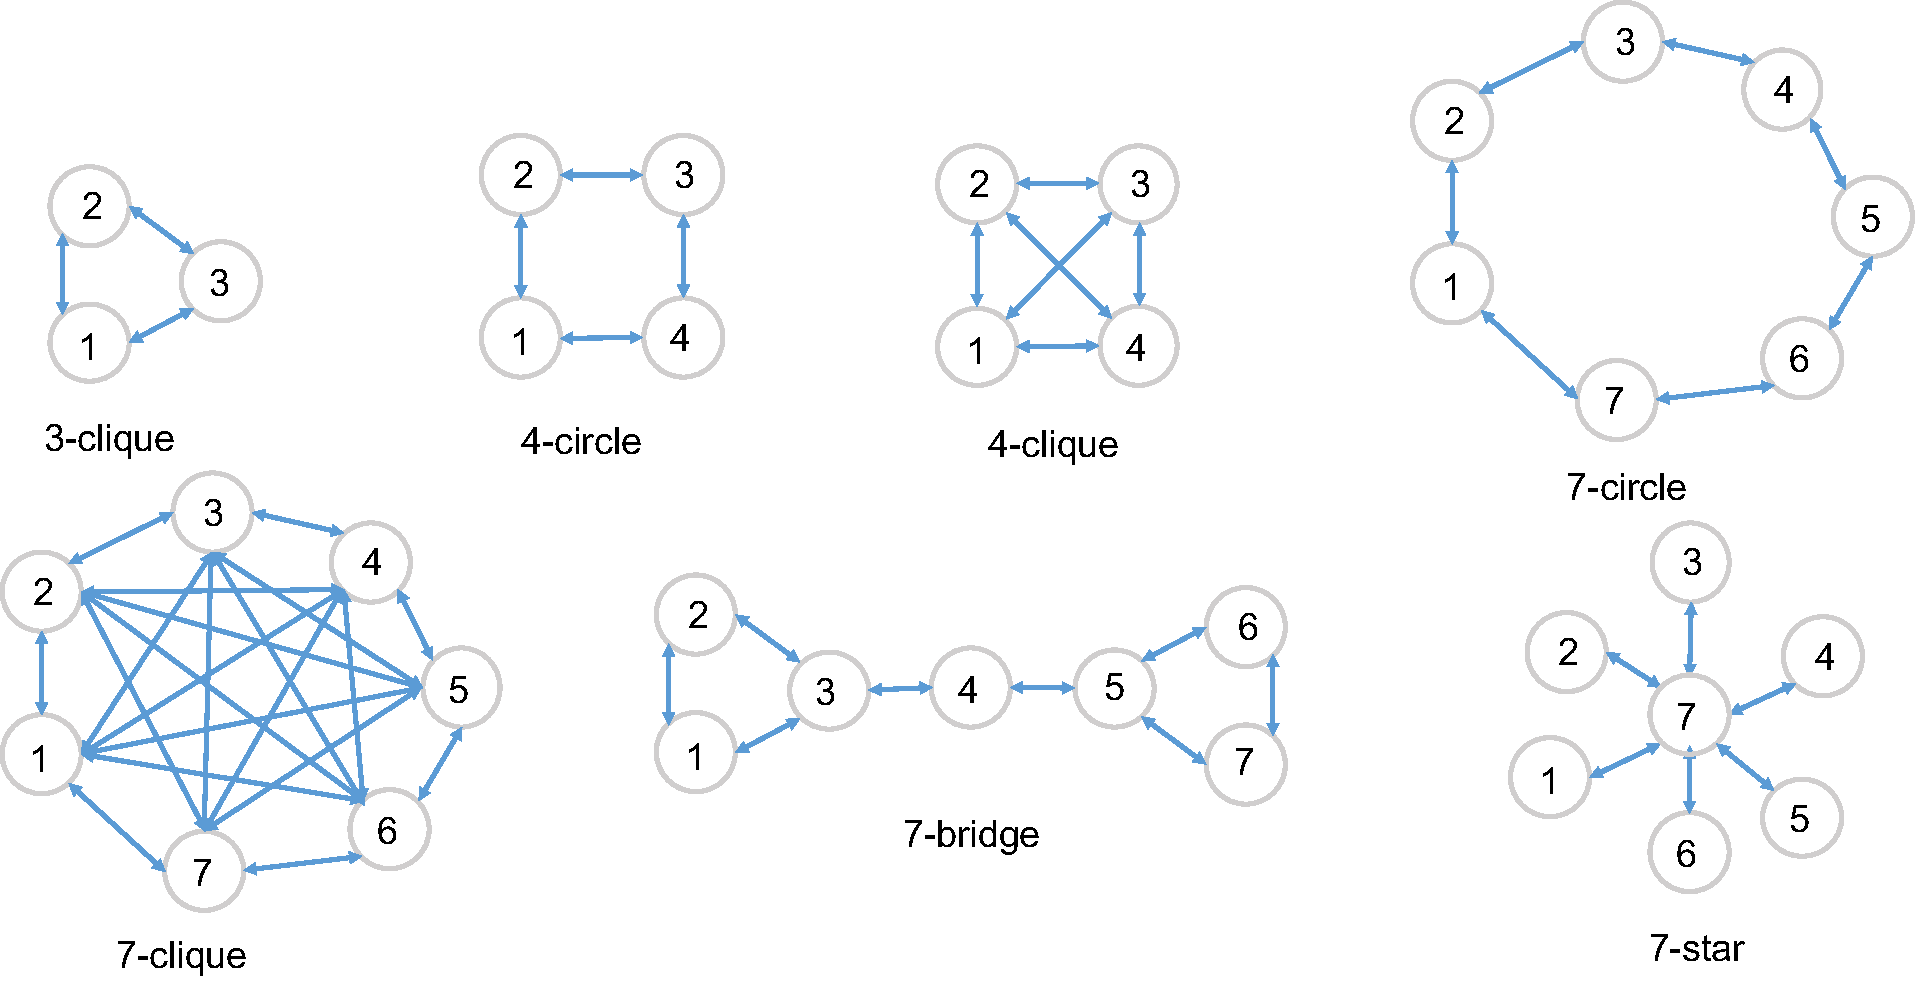
\includegraphics[width=0.75\textwidth]{figures/cluster_set_up.pdf}
    \caption{
        Cluster set up for different network topologies.
     }
\label{cluster_set_up}
\end{center}
\end{figure*}

We have used the AWS cloud services with 7 virtual machines, for each node, it includes a four core AMD EPYC 7571, with 16 Gb of memory size and 296Gb of disk size. 
The JAVA version is 1.8, we have deployed our service using docker and the docker version is 18.02.0-ce.   

We have 7 topologies set up of nodes, which are shown in Figure~\ref{cluster_set_up}, these configurations are aiming to test: 
\begin{itemize}
    \item The performance when the cluster connectivity is high (congestion of communications, like 3-clique, 4-clique, 7-clique and 7-star);
    \item The performance when the cluster diameter is high (long hops to pass message, like 4-circle, 7-circle, 7-bridge);
\end{itemize}

As for the data, we have created 1,000 accounts, with the genesis account having 1,000,000,000 tokens in the coinbase block.
We divided the accounts into two groups (each group will have 500 accounts), the first group will participate in the ramp up step, which means the genesis account will distribute the tokens to these accounts.
And for comparison we have issued four set of different size transactions (5000, 10000, 15000 and 20000) respectively.
In the execution step, the first group of accounts will issue transactions to the second group of accounts, which constructs a bipartite spending graph. 
Since there are more transactions than the number of accounts, there will be double spend manners in this step.
The number of threads in this procedure is equal to the number of nodes for each configuration.
Jmeter \cite{halili2008apache} is utilized as the driver to issue the transactions and 
Nginx \cite{nedelcu2010nginx} is used to evenly and randomly distribute the requests to different nodes.

\subsection {Results and Discussions}

\subsubsection {Block generation rate test}
To test the block generation rate, we set each block in StreamNet to have only one transaction.
And the performance on this configuration is as Figure~\ref{single_txn} shows.
To begin with, as the size of the cluster grows, the network as a whole will witness little performance loss on all of the data scales. 
In the experiment, we can also see that with the growth of the data, the average TPS on most of the configurations have grown a little bit (there are definitely outliers that need our time to triage), 
this is because the genesis forwarding algorithm needs some ramp up time to get to the stable growth stage. 
Considering the system is dealing a growing graph instead of a chain, and the complexity analysis in the previous section,
the experiment clearly shows that our streaming algorithm shed the light on how to deal with the growing DAG.

\begin{figure}[!ht]
\begin{center}
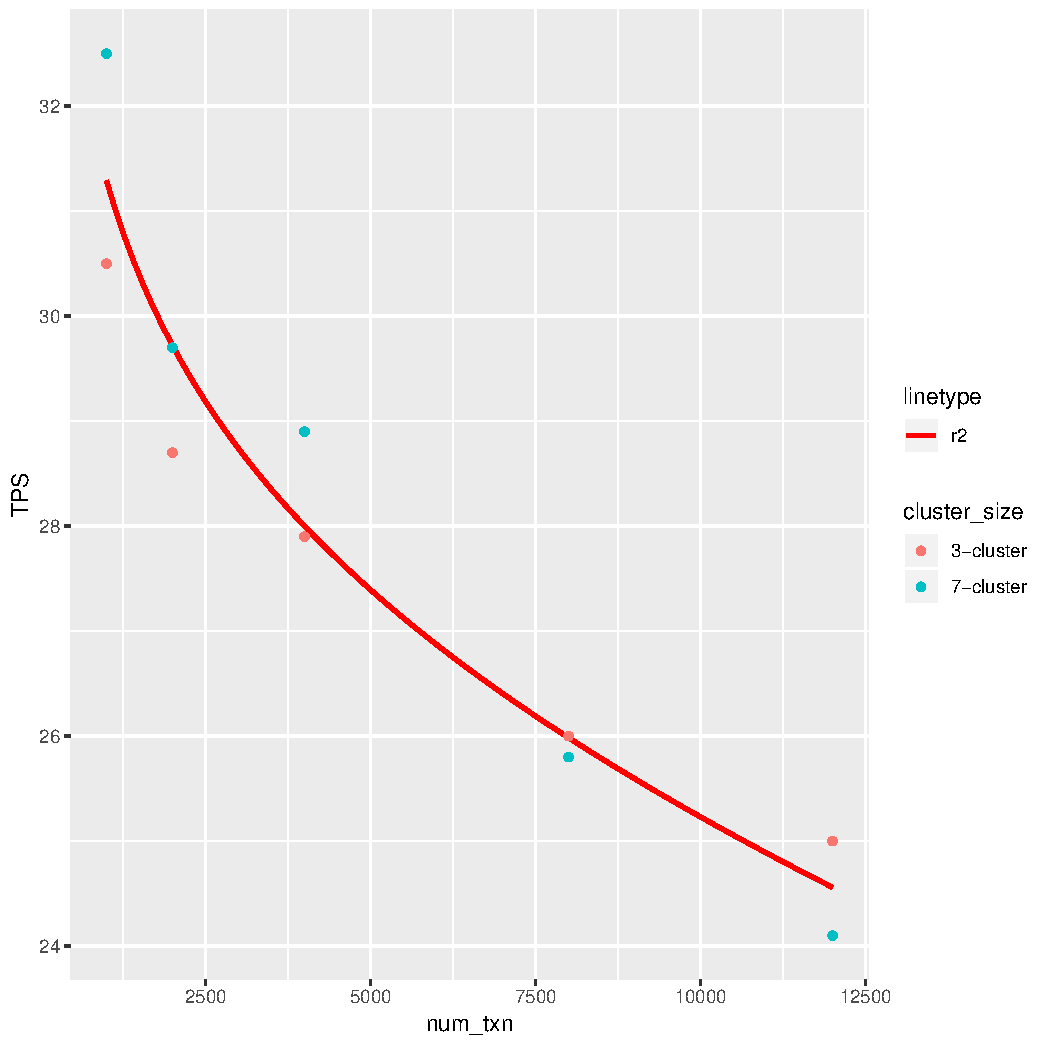
\includegraphics[height=0.35\textwidth, width=0.45\textwidth]{figures/single_txn.pdf}
    \caption{
        Experimental results for block generation rate.
     }
\label{single_txn}
\end{center}
\end{figure}



\subsubsection {Bundle transaction test}

By default, each block in StreamNet will support bundle transaction. 
We set each bundle to contain 20 transactions and for each block there are approximately 3 transactions included.
The performance on this configuration is as Figure~\ref{multi_txn} shows.
In this experiment, we can see that the performance (TPS) comparing with the block test improved more than twice. 
This is because there will be less POW works to be done.
In addition, with growth of the data we do not witness obvious performance down turn. But there are some performance thrashing in the experiment, which needs more study. 

\begin{figure}[!ht]
\begin{center}
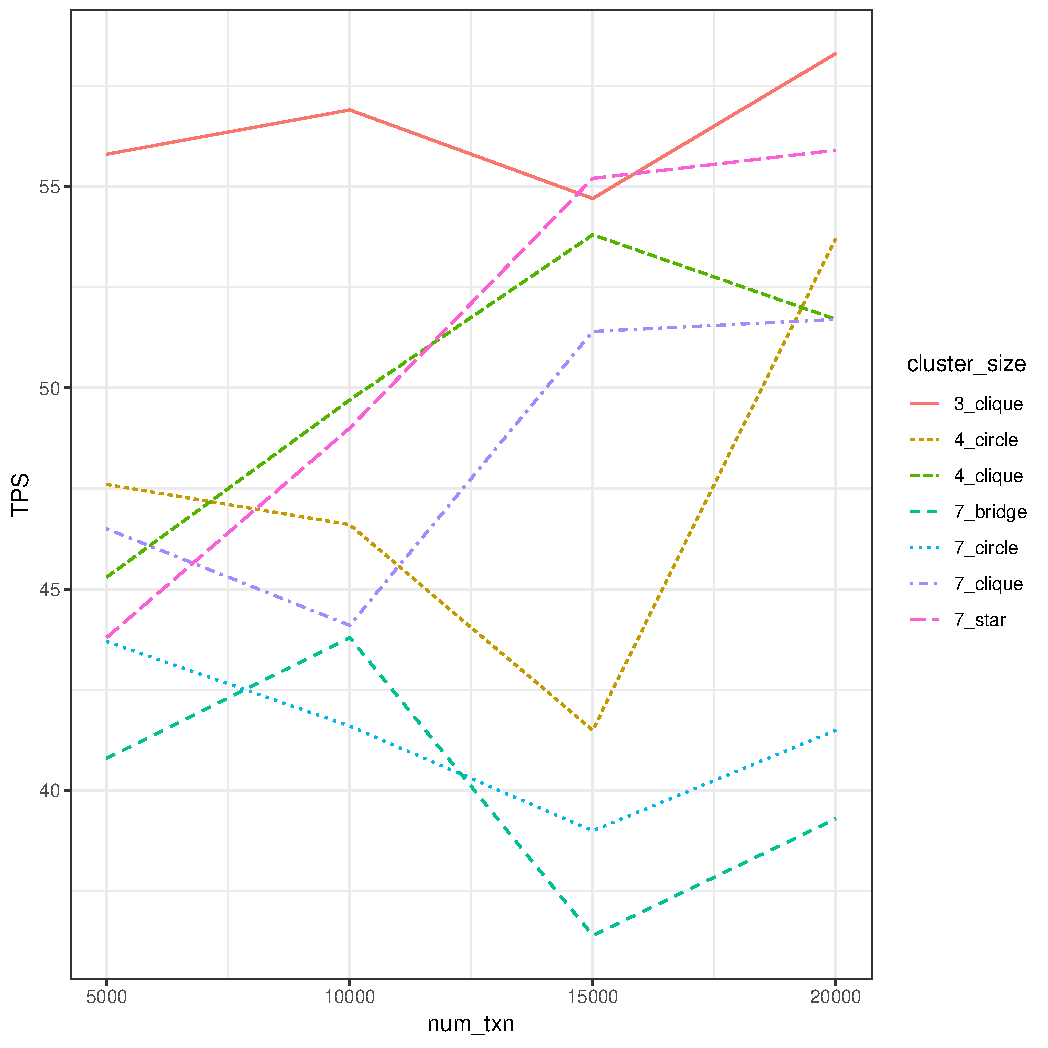
\includegraphics[height=0.35\textwidth, width=0.45\textwidth]{figures/multi_txn.pdf}
    \caption{
        Experimental results for bundle transaction.
     }
\label{multi_txn}
\end{center}
\end{figure}


